% ============================================================
%  پروپوزال رویداد مخابرات کوانتومی - همراه اول
%  کامپایلر: XeLaTeX
% ============================================================
\documentclass[a4paper,12pt]{article}

% ── بسته‌های اصلی ──────────────────────────────────────────
\usepackage{fontspec}

\usepackage{geometry}
\usepackage{xcolor}
\usepackage{graphicx}
\usepackage{tikz}
\usepackage{pgffor}
\usepackage{array}
\usepackage{tabularx}
\usepackage{booktabs}
\usepackage{multirow}
\usepackage{enumitem}
\usepackage{mdframed}
\usepackage{titlesec}
\usepackage{fancyhdr}
\usepackage{hyperref}
\usepackage{eso-pic}   % برای پس‌زمینه صفحه

\usetikzlibrary{shapes.geometric, arrows.meta, positioning, decorations.pathreplacing, calc}

% ── تنظیمات صفحه ──────────────────────────────────────────
\geometry{
	a4paper,
	top=2.5cm, bottom=2.5cm,
	left=2.5cm, right=2.5cm,
	headheight=1.5cm
}

\usepackage{xepersian}

% ── فونت‌ها ────────────────────────────────────────────────
\settextfont{XB Niloofar}
\setdigitfont{XB Niloofar}

% فونت انگلیسی
\newfontfamily\enfont{TeX Gyre Termes}

% ── پالت رنگ (بر پایه هویت همراه اول: آبی عمیق + جزئیات کوانتوم) ─
\definecolor{mci-blue}{HTML}{003A70}      % آبی اصلی همراه اول
\definecolor{mci-accent}{HTML}{0074C8}    % آبی روشن‌تر
\definecolor{mci-gold}{HTML}{C8973A}      % طلایی برای تأکید
\definecolor{mci-light}{HTML}{E8F1FA}     % پس‌زمینه روشن
\definecolor{mci-dark}{HTML}{1A1A2E}      % تیره برای متن روی رنگ
\definecolor{mci-gray}{HTML}{5A6A7A}      % خاکستری متن ثانویه
\definecolor{mci-border}{HTML}{B0C4D8}    % رنگ خطوط

% ── تنظیمات هایپرلینک ─────────────────────────────────────
\hypersetup{
	colorlinks=true,
	linkcolor=mci-blue,
	urlcolor=mci-accent,
	pdfauthor={تیم تحقیق و فناوری همراه اول},
	pdftitle={پروپوزال رویداد مخابرات کوانتومی}
}

% ── سرصفحه و پاصفحه ──────────────────────────────────────
\pagestyle{fancy}
\fancyhf{}
\renewcommand{\headrulewidth}{0.4pt}
\renewcommand{\headrule}{\hbox to\headwidth{\color{mci-blue}\leaders\hrule height \headrulewidth\hfill}}
\fancyhead[R]{\small\color{mci-gray} تیم تحقیق و فناوری - همراه اول}
\fancyhead[L]{\small\color{mci-gray} پروپوزال رویداد کوانتوم}
\fancyfoot[C]{\small\color{mci-gray}\thepage}

% ── عنوان‌بندی بخش‌ها ─────────────────────────────────────
\titleformat{\section}
{\large\bfseries\color{mci-blue}}
{\thesection.}{0.5em}{}
[\textcolor{mci-accent}{\titlerule[1.5pt]}]

\titleformat{\subsection}
{\normalsize\bfseries\color{mci-dark}}
{\thesubsection.}{0.5em}{}

\setlength{\parindent}{0pt}
\setlength{\parskip}{6pt}

% ── دستورات کمکی ─────────────────────────────────────────
\newcommand{\speakercard}[4]{%
	% #1 نام  #2 سمت  #3 دانشگاه  #4 موضوع سخنرانی
	\begin{mdframed}[
		linecolor=mci-border,
		backgroundcolor=mci-light,
		roundcorner=4pt,
		innertopmargin=8pt,
		innerbottommargin=8pt,
		innerleftmargin=10pt,
		innerrightmargin=10pt,
		linewidth=1pt
		]
		{\bfseries\color{mci-blue} #1}\\[2pt]
		{\small\color{mci-gray} #2 \textbar\ #3}\\[4pt]
		{\small\itshape موضوع: #4}
	\end{mdframed}
	\vspace{4pt}
}

% ─────────────────────────────────────────────────────────
\begin{document}
	\settextfont{XB Niloofar}[Script=Arabic]
	
	% ════════════════════════════════════════════════════════
	%  صفحه کاور
	% ════════════════════════════════════════════════════════
	\begin{titlepage}
		
		% پس‌زمینه گرادیان
		\begin{tikzpicture}[remember picture, overlay]
			% نوار بالایی
			\fill[mci-blue]
			(current page.north west) rectangle
			([yshift=-6cm]current page.north east);
			% نوار پایینی باریک
			\fill[mci-accent]
			([yshift=1.2cm]current page.south west) rectangle
			(current page.south east);
			% خطوط تزئینی «مدار کوانتومی»
			\foreach \i in {1,...,6}{
				\draw[mci-accent, opacity=0.15, line width=0.6pt]
				([xshift=\i*1.8cm, yshift=-6cm]current page.north west)
				-- ([xshift=\i*1.8cm]current page.south west);
			}
			% دایره‌های کوانتومی نمادین
			\draw[mci-gold, opacity=0.25, line width=1pt]
			([xshift=3cm, yshift=-3cm]current page.north east) circle (2.5cm);
			\draw[mci-gold, opacity=0.15, line width=0.8pt]
			([xshift=3cm, yshift=-3cm]current page.north east) circle (4cm);
			% لوگو
			\node[anchor=north east] at ([xshift=-1.5cm, yshift=-0.8cm]current page.north east){%
				
\includegraphics[width=6.2cm]{figs/logo-mci-rnd.pdf}
			};
		\end{tikzpicture}
		
		\vspace*{1cm}
		
		% عنوان اصلی روی نوار آبی
		{\color{white}\fontsize{22}{30}\selectfont\bfseries
			\begin{center}
				رویداد تخصصی
			\end{center}
		}
		
		{\color{mci-gold}\fontsize{28}{38}\selectfont\bfseries
			\begin{center}
				مخابرات کوانتومی\\[6pt]
				و رمزنگاری پساکوانتومی
			\end{center}
		}
		
		\vspace{1.2cm}
		
		{\color{white}\large
			\begin{center}
				Quantum Communications \& Post-Quantum Cryptography
			\end{center}
		}
		
		\vspace{3cm}
		
		% کادر اطلاعات رویداد
		\begin{center}
			\begin{tikzpicture}
				\node[
				draw=mci-border,
				fill=white,
				rounded corners=6pt,
				inner sep=16pt,
				text width=14cm,
				align=right
				]{
					\begin{tabular}{r l}
						\textbf{\color{mci-blue}نام رویداد:}   & 
						همایش تخصصی مخابرات کوانتومی و رمزنگاری پساکوانتومی (
						\lr{QCom \& PQC}
						 $1405$) \\[6pt]
						\textbf{\color{mci-blue}تاریخ:}        & $15$ آذر $1405$ ($6$ دسامبر $2026$) \\[6pt]
						\textbf{\color{mci-blue}مکان:}         & سالن همایش‌های ساختمان ستاره ونک \\[6pt]
						\textbf{\color{mci-blue}برگزارکننده:}  & تیم تحقیق و فناوری - همراه اول \\
					\end{tabular}
				};
			\end{tikzpicture}
		\end{center}
		
		\vfill
		
		{\small\color{mci-gray}\centering این سند محرمانه است و صرفاً جهت بررسی داخلی تهیه شده است.}
		
	\end{titlepage}
	
	% ════════════════════════════════════════════════════════
	%  بخش ۱: مقدمه و اهداف
	% ════════════════════════════════════════════════════════
	\section{مقدمه و اهداف رویداد}
	
	تیم تحقیق و فناوری همراه اول در نظر دارد یک رویداد تخصصی یک‌روزه در حوزه
	\textbf{مخابرات کوانتومی} و \textbf{رمزنگاری پساکوانتومی (PQC)} برگزار نماید.
	این رویداد با هدف ایجاد بستری برای تبادل دانش، برندینگ واحد تحقیقات، و معرفی
	دستاوردهای علمی تیم طراحی شده است.
	
	\subsection{اهداف اصلی}
	
	\begin{itemize}[rightmargin=0.5cm, itemsep=4pt]
		\item برندینگ و معرفی تیم تحقیق و فناوری همراه اول در سطح جامعه علمی-فناوری کشور
		\item برگزاری سخنرانی‌های تخصصی با حضور اساتید برجسته دانشگاهی و پژوهشگران
		\item رونمایی رسمی از کتاب ترجمه‌شده توسط تیم.
		\item ایجاد شبکه ارتباطی بین متخصصان صنعت و دانشگاه در حوزه امنیت کوانتومی
		\item آشنایی مخاطبان با الگوریتم‌های مقاوم در برابر کوانتوم و استانداردهای NIST PQC
	\end{itemize}
	
	\subsection{محورهای تخصصی رویداد}
	
	\begin{center}
		\begin{tikzpicture}[
			topic/.style={
				draw=mci-blue, fill=mci-light,
				rounded corners=5pt, text width=5.2cm,
				align=center, minimum height=1.2cm,
				font=\small\bfseries\color{mci-blue}
			},
			node distance=0.5cm and 0.4cm
			]
			\node[topic] (t1) {مخابرات کوانتومی\\{\footnotesize\color{mci-gray}QKD \& Quantum Networks}};
			\node[topic, right=of t1] (t2) {رمزنگاری پساکوانتومی\\{\footnotesize\color{mci-gray}NIST PQC Standards}};
			\node[topic, below=of t1] (t3) {امنیت شبکه پساکوانتومی\\{\footnotesize\color{mci-gray}Network Security}};
			\node[topic, right=of t3] (t4) {الگوریتم‌های مقاوم\\{\footnotesize\color{mci-gray}Lattice, Hash-based, ...}};
		\end{tikzpicture}
	\end{center}
	
	% ════════════════════════════════════════════════════════
	%  بخش ۲: سخنرانان مدعو
	% ════════════════════════════════════════════════════════
	\newpage
	\section{سخنرانان مدعو}
	
	\speakercard
	{دکتر ترانه اقلیدس}
	{دانشیار - رمزنگاری و امنیت اطلاعات}
	{پژوهشکده الکترونیک، دانشگاه صنعتی شریف}
	{گذار به رمزنگاری پساکوانتومی: چالش‌ها و استانداردهای جدید NIST}
	
	\speakercard
	{دکتر جواد صالحی}
	{استاد تمام - مهندسی برق}
	{دانشگاه صنعتی شریف}
	{زیرساخت‌های مخابرات نوری و بسترهای فیبری برای توزیع کلید کوانتومی (QKD)}
	
	\speakercard
	{دکتر علی رضاخانی}
	{دانشیار - فیزیک نظری و اطلاعات کوانتومی}
	{دانشکده فیزیک، دانشگاه صنعتی شریف}
	{مبانی نظری اطلاعات کوانتومی و چشم‌انداز شبکه‌های کوانتومی}
	
	\speakercard
	{محمد رضایی}
	{پژوشگر پسادکتری / مدیر پروژه}
	{مرکز فناوری‌های کوانتومی، دانشگاه صنعتی شریف}
	{پیاده‌سازی عملی پروتکل‌های مخابرات کوانتومی در شبکه‌های مخابراتی کشور}
	
	\speakercard
	{امیر یوسفی}
	{پژوهشگر دکتری}
	{آزمایشگاه فوتونیک و اندازه‌گیری کوانتومی (LPQM)، دانشگاه EPFL سوئیس}
	{فناوری‌های نوین حسگری کوانتومی و کاربردهای صنعتی آن}
	
%	\speakercard
%	{محمد لامعی رشتی}
%	{عضو هیئت علمی پژوهشکده ذرات و شتابگرها}
%	{پژوهشگاه دانش‌های بنیادی (IPM)}
%	{فیزیک کوانتومی در مقیاس بزرگ: از شتابگرها تا فناوری‌های کوانتومی}
%	
	% ════════════════════════════════════════════════════════
	%  بخش ۳: برنامه زمانی - سناریوی اول (با نهار)
	% ════════════════════════════════════════════════════════
	\newpage
	\section{برنامه زمانی - سناریوی اول (با پذیرایی نهار)}
	
	\begin{center}
		{\small\color{mci-gray}زمان کل: $8:30$ تا $17:30$}
	\end{center}
	
	\vspace{0.4cm}
	
	\begin{tikzpicture}[
		slot/.style={
			draw=mci-border, fill=white,
			rounded corners=3pt,
			minimum height=0.9cm,
			text width=12cm,
			inner xsep=8pt, align=right,
			font=\small
		},
		break/.style={
			draw=mci-accent!40, fill=mci-light,
			rounded corners=3pt,
			minimum height=0.9cm,
			text width=12cm,
			inner xsep=8pt, align=right,
			font=\small\color{mci-gray}
		},
		timebox/.style={
			text width=2.8cm, align=left,
			font=\small\bfseries\color{mci-blue}
		}
		]
		
		\def\ypos{0}
		\def\ystep{-1.1}
		
		% ردیف اول - پذیرش
		\node[timebox] at (0,\ypos) {$8:30$ - $9:00$};
		\node[break] at (8,\ypos) {ثبت‌نام و پذیرش شرکت‌کنندگان};
		
		\pgfmathsetmacro\ypos{\ypos+\ystep}
		% افتتاحیه
		\node[timebox] at (0,\ypos) {$9:00$ - $9:30$};
		\node[slot] at (8,\ypos) {\textbf{مراسم افتتاحیه} - معرفی تیم تحقیق و فناوری همراه اول};
		
		\pgfmathsetmacro\ypos{\ypos+\ystep}
		% سخنرانی ۱
		\node[timebox] at (0,\ypos) {$9:30$ - $10:15$};
		\node[slot] at (8,\ypos) {\textbf{سخنرانی اول} - گذار به رمزنگاری پساکوانتومی \textbar\ دکتر ترانه اقلیدس};
		
		\pgfmathsetmacro\ypos{\ypos+\ystep}
		% سخنرانی ۲
		\node[timebox] at (0,\ypos) {$10:15$ - $11:00$};
		\node[slot] at (8,\ypos) {\textbf{سخنرانی دوم} - زیرساخت‌های مخابرات نوری و QKD \textbar\ دکتر جواد صالحی};
		
		\pgfmathsetmacro\ypos{\ypos+\ystep}
		% استراحت صبح
		\node[timebox] at (0,\ypos) {$11:00$ - $11:20$};
		\node[break] at (8,\ypos) {پذیرایی - استراحت};
		
		\pgfmathsetmacro\ypos{\ypos+\ystep}
		% سخنرانی ۳
		\node[timebox] at (0,\ypos) {$11:20$ - $12:05$};
		\node[slot] at (8,\ypos) {\textbf{سخنرانی سوم} - مبانی نظری اطلاعات کوانتومی \textbar\ دکتر علی رضاخانی};
		
		\pgfmathsetmacro\ypos{\ypos+\ystep}
		% نهار
		\node[timebox] at (0,\ypos) {$12:05$ - $13:30$};
		\node[break] at (8,\ypos) {ناهار و نماز};
		
		\pgfmathsetmacro\ypos{\ypos+\ystep}
		% رونمایی کتاب
		\node[timebox] at (0,\ypos) {$13:30$ - $14:15$};
		\node[slot,draw=mci-gold,fill=mci-gold!8] at (8,\ypos)
		{\textbf{\color{mci-gold}رونمایی از کتاب} - ارتباطات کوانتومی، شبکه‌های کوانتومی و حسگری کوانتومی};
		
		\pgfmathsetmacro\ypos{\ypos+\ystep}
		% سخنرانی ۴
		\node[timebox] at (0,\ypos) {$14:15$ - $15:00$};
		\node[slot] at (8,\ypos) {\textbf{سخنرانی چهارم} - پیاده‌سازی عملی پروتکل‌های کوانتومی \textbar\ محمد رضایی};
		
		\pgfmathsetmacro\ypos{\ypos+\ystep}
		% سخنرانی ۵
		\node[timebox] at (0,\ypos) {$15:00$ - $15:45$};
		\node[slot] at (8,\ypos) {\textbf{سخنرانی پنجم} - فناوری‌های نوین حسگری کوانتومی \textbar\ امیر یوسفی};
		
		\pgfmathsetmacro\ypos{\ypos+\ystep}
		% استراحت بعدازظهر
		\node[timebox] at (0,\ypos) {$15:45$ - $16:00$};
		\node[break] at (8,\ypos) {پذیرایی - استراحت};
		
		\pgfmathsetmacro\ypos{\ypos+\ystep}
		% سخنرانی ۶
		\node[timebox] at (0,\ypos) {$16:00$ - $16:45$};
		\node[slot] at (8,\ypos) {\textbf{سخنرانی ششم} - فیزیک کوانتومی در مقیاس بزرگ \textbar\ محمد لامعی رشتی};
		
		\pgfmathsetmacro\ypos{\ypos+\ystep}
		% اختتامیه
		\node[timebox] at (0,\ypos) {$16:45$ - $17:30$};
		\node[slot,fill=mci-blue!8,draw=mci-blue] at (8,\ypos)
		{\textbf{\color{mci-blue}اختتامیه} - جمع‌بندی، پرسش و پاسخ، عکس یادگاری};
		
	\end{tikzpicture}
	
	% ════════════════════════════════════════════════════════
	%  بخش ۴: برنامه زمانی - سناریوی دوم (بدون نهار)
	% ════════════════════════════════════════════════════════
	\newpage
	\section{برنامه زمانی - سناریوی دوم (بدون پذیرایی نهار)}
	
	\begin{center}
		{\small\color{mci-gray}زمان کل: $8:30$ تا $13:30$}
	\end{center}
	
	\vspace{0.4cm}
	
	\begin{center}
		\begin{tikzpicture}[
			slot/.style={
				draw=mci-border, fill=white,
				rounded corners=3pt, minimum height=0.9cm,
				text width=12cm, inner xsep=8pt, align=right,
				font=\small
			},
			break/.style={
				draw=mci-accent!40, fill=mci-light,
				rounded corners=3pt, minimum height=0.9cm,
				text width=12cm, inner xsep=8pt, align=right,
				font=\small\color{mci-gray}
			},
			timebox/.style={
				text width=2.8cm, align=left,
				font=\small\bfseries\color{mci-blue}
			}
			]
			
			\def\ypos{0}
			\def\ystep{-1.1}
			
			\node[timebox] at (0,\ypos) {$8:30$ - $9:00$};
			\node[break] at (8,\ypos) {ثبت‌نام و پذیرش شرکت‌کنندگان};
			
			\pgfmathsetmacro\ypos{\ypos+\ystep}
			\node[timebox] at (0,\ypos) {$9:00$ - $9:20$};
			\node[slot] at (8,\ypos) {\textbf{مراسم افتتاحیه} - معرفی تیم تحقیق و فناوری};
			
			\pgfmathsetmacro\ypos{\ypos+\ystep}
			\node[timebox] at (0,\ypos) {$9:20$ - $10:00$};
			\node[slot] at (8,\ypos) {\textbf{سخنرانی اول} - گذار به رمزنگاری پساکوانتومی \textbar\ دکتر ترانه اقلیدس};
			
			\pgfmathsetmacro\ypos{\ypos+\ystep}
			\node[timebox] at (0,\ypos) {$10:00$ - $10:40$};
			\node[slot] at (8,\ypos) {\textbf{سخنرانی دوم} - زیرساخت‌های مخابرات نوری و QKD \textbar\ دکتر جواد صالحی};
			
			\pgfmathsetmacro\ypos{\ypos+\ystep}
			\node[timebox] at (0,\ypos) {$10:40$ - $11:00$};
			\node[break] at (8,\ypos) {پذیرایی - استراحت};
			
			\pgfmathsetmacro\ypos{\ypos+\ystep}
			\node[timebox] at (0,\ypos) {$11:00$ - $11:40$};
			\node[slot] at (8,\ypos) {\textbf{سخنرانی سوم} - مبانی نظری اطلاعات کوانتومی \textbar\ دکتر علی رضاخانی};
			
			\pgfmathsetmacro\ypos{\ypos+\ystep}
			\node[timebox] at (0,\ypos) {$11:40$ - $12:20$};
			\node[slot] at (8,\ypos) {\textbf{سخنرانی چهارم} - پیاده‌سازی عملی پروتکل‌های کوانتومی \textbar\ محمد رضایی};
			
			\pgfmathsetmacro\ypos{\ypos+\ystep}
			\node[timebox] at (0,\ypos) {$12:20$ - $13:00$};
			\node[slot,draw=mci-gold,fill=mci-gold!8] at (8,\ypos)
			{\textbf{\color{mci-gold}رونمایی از کتاب} - ارتباطات کوانتومی، شبکه‌های کوانتومی و حسگری کوانتومی};
			
			\pgfmathsetmacro\ypos{\ypos+\ystep}
			\node[timebox] at (0,\ypos) {$13:00$ - $13:30$};
			\node[slot,fill=mci-blue!8,draw=mci-blue] at (8,\ypos)
			{\textbf{\color{mci-blue}اختتامیه} - جمع‌بندی، پرسش و پاسخ};
			
		\end{tikzpicture}
	\end{center}
	
	% ════════════════════════════════════════════════════════
	%  بخش ۵: معرفی کتاب
	% ════════════════════════════════════════════════════════
	\newpage
	\section{معرفی کتاب}
	
	\begin{mdframed}[
		linecolor=mci-gold,
		linewidth=2pt,
		backgroundcolor=mci-gold!5,
		roundcorner=6pt,
		innertopmargin=14pt,
		innerbottommargin=14pt,
		innerleftmargin=14pt,
		innerrightmargin=14pt
		]
		
		\begin{minipage}{0.2\textwidth}
			\centering
			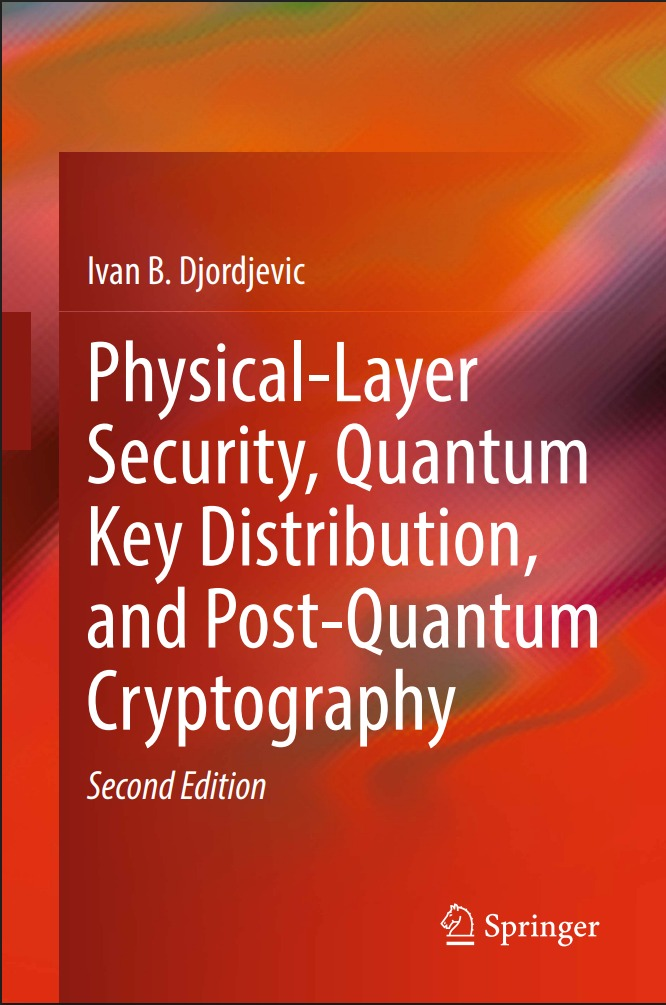
\includegraphics[width=\linewidth]{figs/book}
		\end{minipage}
		\hfill
		\begin{minipage}{0.76\textwidth}
			\textbf{\large\color{mci-blue}
				\rl{
					ارتباطات کوانتومی،
					شبکه‌های کوانتومی و
					حسگری کوانتومی
			}}
			\\[4pt]
			{\footnotesize\color{mci-gray}\lr{
					Quantum Communication,
					Quantum Networks, and
					Quantum Sensing
			}}\\[8pt]
			\textbf{مترجمان:} \rl{
				محمد رضیئی، اسماعیل اسکندری
			}\\[4pt]
			\textbf{ناشر:} انتشارات جهاد دانشگاهی امیرکبیر\\[4pt]
			\textbf{سال انتشار:} $1405$\\[8pt]
			{\small این کتاب توسط اعضای تیم تحقیق و فناوری همراه اول ترجمه شده
				و یکی از منابع اصلی آموزشی در حوزه 
				\textit{مخابرات کوانتومی}
				محسوب می‌شود.}
		\end{minipage}
		
	\end{mdframed}
	
	% ════════════════════════════════════════════════════════
	%  بخش ۶: اطلاعات مخاطبان هدف و مشخصات اجرایی
	% ════════════════════════════════════════════════════════
	\section{مخاطبان هدف}
	
	\begin{itemize}[rightmargin=0.5cm, itemsep=3pt]
		\item متخصصان حوزه مخابرات و امنیت اطلاعات در شرکت‌های فناوری
		\item دانشجویان و پژوهشگران دانشگاهی در رشته‌های مرتبط
		\item مدیران و تصمیم‌گیرندگان حوزه امنیت سایبری
		\item علاقه‌مندان به فناوری‌های نوظهور کوانتومی
	\end{itemize}
	
	\section{مشخصات اجرایی}
	
	\begin{tabularx}{\textwidth}{>{\bfseries\color{mci-blue}}r X}
		\toprule
		مکان برگزاری & سالن همایش‌های ساختمان ستاره ونک \\
		\midrule
		ظرفیت تخمینی & $150$ نفر \\
		\midrule
		زبان رویداد & فارسی (با اسلایدهای انگلیسی) \\
		\midrule
		ضبط و پخش & حضوری با پخش زنده آنلاین \\
		\midrule
		هزینه ثبت‌نام & رایگان (با ثبت‌نام و تأیید قبلی) \\
		\bottomrule
	\end{tabularx}
	
	% ════════════════════════════════════════════════════════
	%  پیوست: معرفی سخنرانان و دلیل انتخاب
	% ════════════════════════════════════════════════════════
	\newpage
	\section*{پیوست الف: معرفی سخنرانان و دلیل انتخاب ایشان}
	\addcontentsline{toc}{section}{پیوست الف: معرفی سخنرانان و دلیل انتخاب ایشان}
	
	{\small\color{mci-gray}
		در ادامه، معرفی مختصری از هر یک از سخنرانان مدعو به همراه دلیل انتخاب ایشان
		برای این رویداد آمده است. اطلاعات مربوط به سخنرانان بر اساس منابع عمومی
		در دسترس و سوابق پژوهشی ایشان تنظیم شده است.}
	
	\vspace{6pt}
	
	\newcommand{\speakerprofile}[5]{%
		% #1 نام  #2 عکس/جای‌نگه‌دار  #3 سمت و وابستگی  #4 معرفی  #5 دلیل انتخاب
		\begin{mdframed}[
			linecolor=mci-border,
			backgroundcolor=white,
			roundcorner=5pt,
			innertopmargin=10pt,
			innerbottommargin=10pt,
			innerleftmargin=12pt,
			innerrightmargin=12pt,
			linewidth=1pt
			]
			\begin{minipage}[t]{0.22\textwidth}
				\centering
				#2
			\end{minipage}
			\hfill
			\begin{minipage}[t]{0.73\textwidth}
				{\bfseries\large\color{mci-blue} #1}\\[2pt]
				{\small\color{mci-gray} #3}\\[6pt]
				{\small #4}\\[6pt]
				{\small\color{mci-dark}\textbf{دلیل انتخاب: } #5}
			\end{minipage}
		\end{mdframed}
		\vspace{8pt}
	}
	
	\speakerprofile
	{دکتر ترانه اقلیدس}
	{\raisebox{-3.5cm}{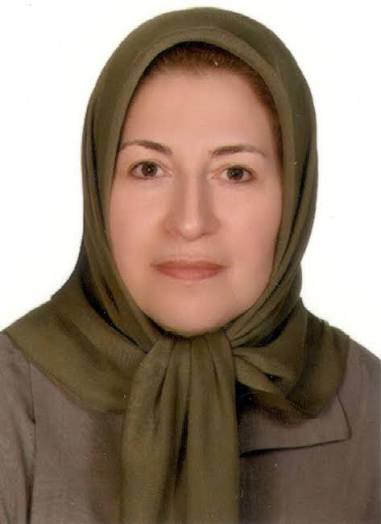
\includegraphics[width=2.5cm]{figs/oghlidus.jpeg}}}
	{دانشیار پژوهشکده الکترونیک، دانشگاه صنعتی شریف}
	{ایشان به‌عنوان نماینده کمیته علمی انجمن رمز ایران در دانشگاه صنعتی شریف فعالیت داشته و از چهره‌های شناخته‌شده جامعه رمزنگاری کشور محسوب می‌شوند.}
	{با توجه به سابقه فعالیت در انجمن رمز ایران، ایشان می‌توانند دیدگاهی جامع و به‌روز از وضعیت رمزنگاری کلاسیک و مسیر گذار به رمزنگاری پساکوانتومی در سطح ملی ارائه دهند؛ موضوعی که هسته اصلی این رویداد را تشکیل می‌دهد.}
	
	\speakerprofile
	{دکتر جواد صالحی}
	{\raisebox{-3.5cm}{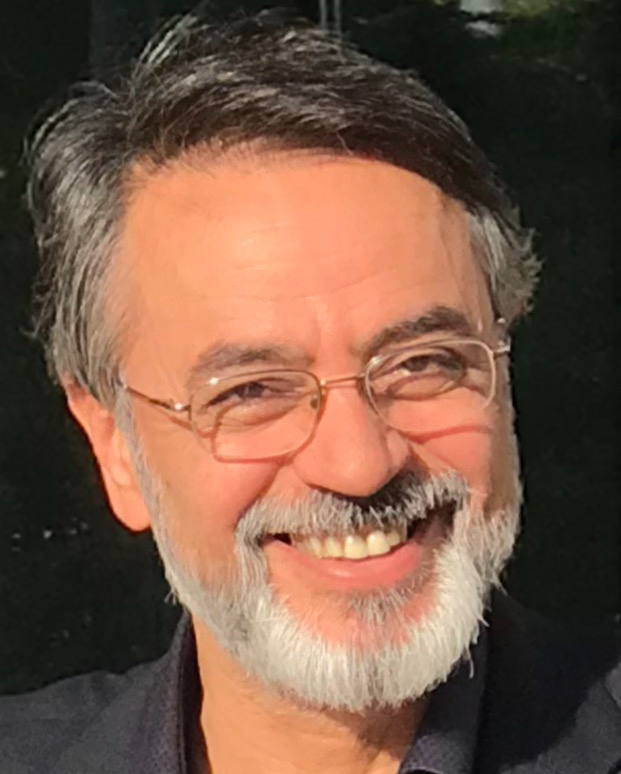
\includegraphics[width=2.5cm]{figs/salehi.jpg}}}
	{استاد تمام، دانشکده مهندسی برق، دانشگاه صنعتی شریف}
	{دکترای مخابرات را از دانشگاه کالیفرنیای جنوبی (USC) اخذ کرده و پیش از بازگشت به ایران، عضو کادر فنی گروه تحقیقات کاربردی آزمایشگاه‌های بل و پژوهشگر مهمان آزمایشگاه اطلاعات و سامانه‌های تصمیم‌گیری دانشگاه MIT بوده‌اند. زمینه فعالیت ایشان طراحی و ساخت سامانه‌های انتقال نوری و شبکه‌های نسل جدید مخابراتی است.}
	{پیشینه چندین‌ساله ایشان در مخابرات نوری و شبکه‌های داده - به‌عنوان زیرساخت فیزیکی توزیع کلید کوانتومی (QKD) - ایشان را به گزینه‌ای مناسب برای اتصال مباحث نظری مخابرات کوانتومی به واقعیت‌های مهندسی شبکه در کشور تبدیل می‌کند.}
	
	\speakerprofile
	{دکتر علی رضاخانی}
	{\raisebox{-3.5cm}{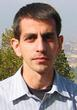
\includegraphics[width=2.5cm]{figs/rezakhani.jpg}}}
	{دانشیار دانشکده فیزیک، دانشگاه صنعتی شریف}
	{دکترای فیزیک (نظریه اطلاعات کوانتومی) را از دانشگاه صنعتی شریف اخذ کرده و دوره‌های فوق‌دکتری را در بنیاد پژوهشی ISI تورین (ایتالیا)، دانشگاه کلگری (کانادا) و دانشگاه کالیفرنیای جنوبی (USC) گذرانده‌اند. زمینه‌های پژوهشی ایشان شامل علوم اطلاعات کوانتومی، محاسبات کوانتومی، سامانه‌های کوانتومی باز، ترمودینامیک و کنترل کوانتومی است.}
	{تخصص مستقیم ایشان در نظریه اطلاعات کوانتومی، دقیقاً هم‌راستا با محور «مخابرات کوانتومی» رویداد است و می‌تواند مبانی نظری لازم برای درک الگوریتم‌ها و پروتکل‌های ارائه‌شده توسط سایر سخنرانان را فراهم کند.}
	
	\speakerprofile
	{محمد رضایی}
	{\raisebox{-3.5cm}{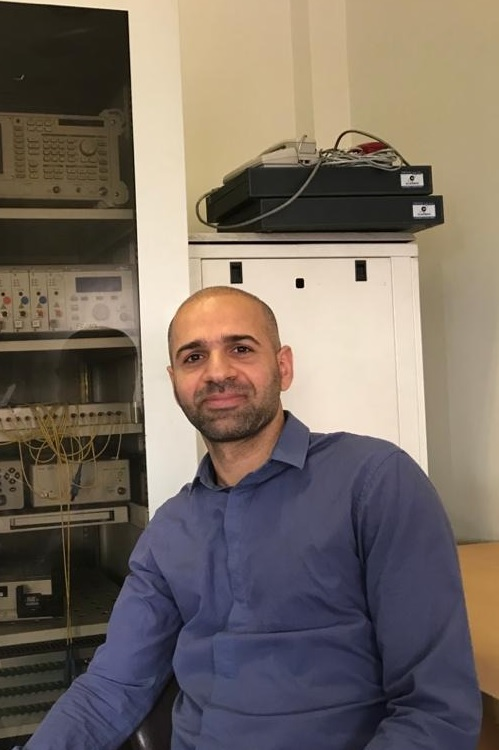
\includegraphics[width=2.5cm]{figs/rezaei.jpg}}}
	{مرکز فناوری‌های کوانتومی، دانشگاه صنعتی شریف}
	{ایشان پژوهشگر فعال در حوزه پیاده‌سازی عملی پروتکل‌های مخابرات کوانتومی و عضو مرکز کوانتوم دانشگاه صنعتی شریف هستند. تمرکز پژوهشی ایشان بر روی یکپارچه‌سازی فناوری‌های کوانتومی با زیرساخت‌های مخابراتی موجود است.}
	{با توجه به تجربه عملی ایشان در پیاده‌سازی سیستم‌های کوانتومی، می‌توانند دیدگاهی کاربردی و معطوف به صنعت در مورد چالش‌های استقرار این فناوری در شبکه‌های مخابراتی کشور ارائه دهند.}
	
	\speakerprofile
	{امیر یوسفی}
	{\raisebox{-1.5cm}{
\includegraphics[width=2.5cm]{figs/yusefi.jpeg}}}
	{آزمایشگاه فوتونیک و اندازه‌گیری کوانتومی (LPQM)، دانشگاه EPFL سوئیس}
	{ایشان پژوهشگر دکتری در دانشگاه پلی‌تکنیک فدرال لوزان (EPFL) سوئیس بوده و در زمینه حسگری کوانتومی، مدارهای ابررسانا و اندازه‌گیری‌های کوانتومی فعالیت می‌کنند.}
	{حضور ایشان از یک مرکز پیشرو اروپایی در فناوری‌های کوانتومی مانند EPFL می‌تواند دیدگاهی بین‌المللی و مقایسه‌ای به رویداد اضافه کند و جدیدترین دستاوردهای جهانی در حوزه حسگری کوانتومی را به مخاطبان معرفی نماید.}
	
	\speakerprofile
	{محمد لامعی رشتی}
	{\raisebox{-2.5cm}{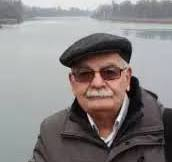
\includegraphics[width=2.5cm]{figs/rashti.jpeg}}}
	{پژوهشکده ذرات و شتابگرها، پژوهشگاه دانش‌های بنیادی (IPM)}
	{ایشان از پیشکسوتان و اعضای هیئت علمی پژوهشگاه دانش‌های بنیادی (IPM) هستند که سابقه‌ای درخشان در طراحی و ساخت شتاب‌دهنده‌های ذرات و پروژه‌های بزرگ فیزیک تجربی در کشور دارند.}
	{تجربه ایشان در مدیریت پروژه‌های بزرگ فیزیک، الگوی مناسبی برای توسعه زیرساخت‌های کوانتومی در سطح ملی ارائه می‌دهد و بُعد آکادمیک و بنیادین رویداد را به‌شکل چشمگیری تقویت می‌کند.}
	
	% ════════════════════════════════════════════════════════
	%  صفحه پایانی
	% ════════════════════════════════════════════════════════
	\newpage
	\thispagestyle{empty}
	
	\begin{tikzpicture}[remember picture, overlay]
		\fill[mci-blue]
		(current page.north west) rectangle
		([yshift=-4cm]current page.north east);
		\fill[mci-accent]
		([yshift=1.2cm]current page.south west) rectangle
		(current page.south east);
	\end{tikzpicture}
	
	\vspace*{1.5cm}
	{\color{white}\Large\bfseries\centering با سپاس از توجه شما}
	
	\vspace{2cm}
	
	\begin{center}
		\begin{mdframed}[
			linecolor=mci-border,
			backgroundcolor=mci-light,
			roundcorner=6pt,
			innertopmargin=16pt, innerbottommargin=16pt,
			innerleftmargin=20pt, innerrightmargin=20pt
			]
			{\large\bfseries\color{mci-blue} شرکت تحقیق و نوآوری}\\[4pt]
			{\color{mci-gray} شرکت ارتباطات سیار ایران (همراه اول)}\\[12pt]
			\textbf{وبسایت:} \url{https://mci.ir/web/rd}\\[4pt]
			
\includegraphics[width=4cm]{figs/logo-mci-rnd.pdf}
		\end{mdframed}
	\end{center}
	
\end{document}